\chapter{画像と文字を扱う}
\label{chap:images-and-text}

この章では、p5.jsで文字と画像を表示する方法を学びます。これまでの章では、円、四角形、線、色、アニメーション、クラスを使って画面を作ってきました。作品らしい見た目にするには、図形だけでなく、タイトル、説明文、得点表示、画像素材などを組み合わせることが重要になります。

\section{この章の概要}

この章では、文字列の表示、フォント、画像の読み込み、画像の表示を扱います。ファイル保存やネットワーク上の画像の読み込みは、ファイル入出力や非同期処理に近い話題になるため、この章では扱いません。

この章で扱う主な内容は次の通りです。

\begin{itemize}
    \item \texttt{string}型の値を画面に表示する方法
    \item \texttt{textSize}、\texttt{textAlign}、\texttt{textWidth}
    \item 文字列を動かす方法
    \item \texttt{p5.Image}型の変数に画像を読み込む方法
    \item \texttt{image}と\texttt{imageMode}
    \item 画像と文字を組み合わせる方法
\end{itemize}

\section{文字列を表示する}

TypeScriptでは、文字列の型を\texttt{string}と書きます。画面に文字を表示するときは、p5.jsの\texttt{text}を使います。文字の色は\texttt{fill}で指定し、文字の大きさは\texttt{textSize}で指定します。

\begin{listing}[htbp]
\inputminted{ts}{listings/chapter12/basic-text.ts}
\caption{文字列を画面に表示する}
\label{lst:chapter12-basic-text}
\end{listing}

このサンプルでは、\texttt{message: string}という定数に文字列を保存しています。\texttt{p.text(message, 40, 80)}は、\texttt{message}の内容を座標\texttt{(40, 80)}に表示します。

\begin{pointbox}{文字も図形と同じように描く}
文字は特別な部品のように見えますが、p5.jsでは図形と同じく\texttt{draw}の中で描画します。\texttt{fill}、\texttt{textSize}、\texttt{textAlign}のような設定は、その後に描く文字に影響します。
\end{pointbox}

\section{文字の位置と整列}

\texttt{text}に4つの数値を渡すと、文字を表示する長方形の領域を指定できます。その領域の中で文字をどのように揃えるかは、\texttt{textAlign}で指定します。

\begin{listing}[htbp]
\inputminted{ts}{listings/chapter12/text-align-box.ts}
\caption{長方形の領域に文字を中央揃えで表示する}
\label{lst:chapter12-text-align-box}
\end{listing}

\texttt{p.textAlign(p.CENTER, p.CENTER)}は、文字を横方向にも縦方向にも中央揃えで表示する設定です。続く\texttt{p.text(message, boxX, boxY, boxWidth, boxHeight)}では、長方形の領域の中に文字を表示しています。

\begin{center}
\begin{tabular}{ll}
\toprule
指定 & 意味 \\
\midrule
\texttt{p.LEFT} & 左揃え \\
\texttt{p.CENTER} & 中央揃え \\
\texttt{p.RIGHT} & 右揃え \\
\texttt{p.TOP} & 上揃え \\
\texttt{p.BOTTOM} & 下揃え \\
\bottomrule
\end{tabular}
\end{center}

\begin{notebox}{文字の座標は図形と少し違う}
\texttt{text}で2つの数値だけを指定した場合、その座標は文字の左下付近の基準線を表します。一方、長方形の領域を指定し、\texttt{textAlign}を使うと、領域の中で文字の位置を考えやすくなります。
\end{notebox}

\section{文字列を動かす}

文字列も、円や四角形と同じように座標を変えれば動かせます。ここでは、文字列が画面の右から左へ流れる例を見ます。

\begin{listing}[htbp]
\inputminted{ts}{listings/chapter12/moving-text.ts}
\caption{\texttt{textWidth}を使って文字列を画面外で戻す}
\label{lst:chapter12-moving-text}
\end{listing}

\texttt{p.textWidth(message)}は、現在の文字設定で\texttt{message}を表示したときの幅を返します。文字列の右端が画面の左端より外に出たら、\texttt{messageX}を\texttt{p.width}に戻しています。

\begin{pointbox}{文字列の幅を使う}
文字列は、内容や文字サイズによって幅が変わります。\texttt{textWidth}を使うと、「文字列が完全に画面から消えたかどうか」を判定できます。
\end{pointbox}

\section{画像を読み込む}

画像を表示するには、まず画像ファイルを読み込み、そのあと画面に描画します。\texttt{let picture: p5.Image;}は、読み込んだ画像を保存する変数の宣言です。\texttt{p.loadImage(...)}の結果を\texttt{picture}へ代入します。

\texttt{picture}は\texttt{p.setup}と\texttt{p.draw}の両方で使うため、これらの関数の外側に宣言しておきます。画像の読み込みには時間がかかる場合があるため、サンプルでは\texttt{p.setup}に\texttt{async}を付け、\texttt{await p.loadImage(...)}で読み込みが終わるのを待っています。\texttt{await}は、読み込みが終わるまで次の行へ進まないようにする書き方です。

\texttt{async}は、その関数の中で\texttt{await}を使えるようにする指定です。戻り値の型\texttt{Promise<void>}は、「処理はあとで完了し、完了時に値を返さない」ことを表します。ここでは、画像を読み込むときに\texttt{async}と\texttt{await}を使う流れを確認します。具体例は、サンプル\ref{lst:chapter12-load-image-basic}を見てください。

\begin{pointbox}{非同期処理は定型として使う}
この章の目標は、\texttt{async}、\texttt{await}、\texttt{Promise<void>}の仕組みを完全に理解することではありません。これらは、画像ファイルの読み込みが終わるのを待つために必要な定型として使います。まずは\texttt{p.setup = async (): Promise<void> => \{ ... \};}と\texttt{await p.loadImage(...)}をひとまとまりとして読み、画像を読み込んで表示する流れに注目してください。
\end{pointbox}

\begin{listing}[htbp]
\inputminted{ts}{listings/chapter12/load-image-basic.ts}
\caption{\texttt{loadImage}関数で画像を読み込んで表示する}
\label{lst:chapter12-load-image-basic}
\end{listing}

このサンプルでは、\texttt{let picture: p5.Image;}で宣言した変数に、\texttt{await p.loadImage("images/sample.png")}で読み込んだ画像を保存しています。

\begin{notebox}{画像ファイルの置き場所}
この章のサンプルでは、画像ファイルを\texttt{images/sample.png}として読み込む想定にしています。実際のプロジェクトでは、開発用サーバから見える場所に画像を置き、パスの文字列と実際のファイル名を一致させる必要があります。
\end{notebox}

\section{画像の大きさと表示位置}

\texttt{image}には、画像、x座標、y座標だけでなく、表示する幅と高さも指定できます。また、\texttt{imageMode}を使うと、座標を左上として扱うか、中心として扱うかを変えられます。
また、\texttt{p5.Image}型の変数は元の大きさを保持しているため、
表示する幅と高さを指定しない場合は、元の大きさで表示されます。
保存されている画像の大きさを知りたい場合は、幅は\texttt{width}、高さは\texttt{height}で取得できます。
具体例は、サンプル\ref{lst:chapter12-image-size-and-mode}を見てください。

\begin{listing}[htbp]
\inputminted{ts}{listings/chapter12/image-size-and-mode.ts}
\caption{\texttt{imageMode}と表示サイズを指定する}
\label{lst:chapter12-image-size-and-mode}
\end{listing}

\texttt{p.imageMode(p.CORNER)}では、指定した座標が画像の左上になります。\texttt{p.imageMode(p.CENTER)}では、指定した座標が画像の中心になります。これは、\texttt{rectMode}とよく似た考え方です。

\begin{center}
\begin{tabular}{ll}
\toprule
書き方 & 意味 \\
\midrule
\texttt{p.image(picture, x, y)} & 元の大きさで表示する \\
\texttt{p.image(picture, x, y, w, h)} & 幅\texttt{w}、高さ\texttt{h}で表示する \\
\texttt{p.imageMode(p.CORNER)} & 座標を画像の左上として扱う \\
\texttt{p.imageMode(p.CENTER)} & 座標を画像の中心として扱う \\
\bottomrule
\end{tabular}
\end{center}

\begin{figure}[htbp]
    \centering
    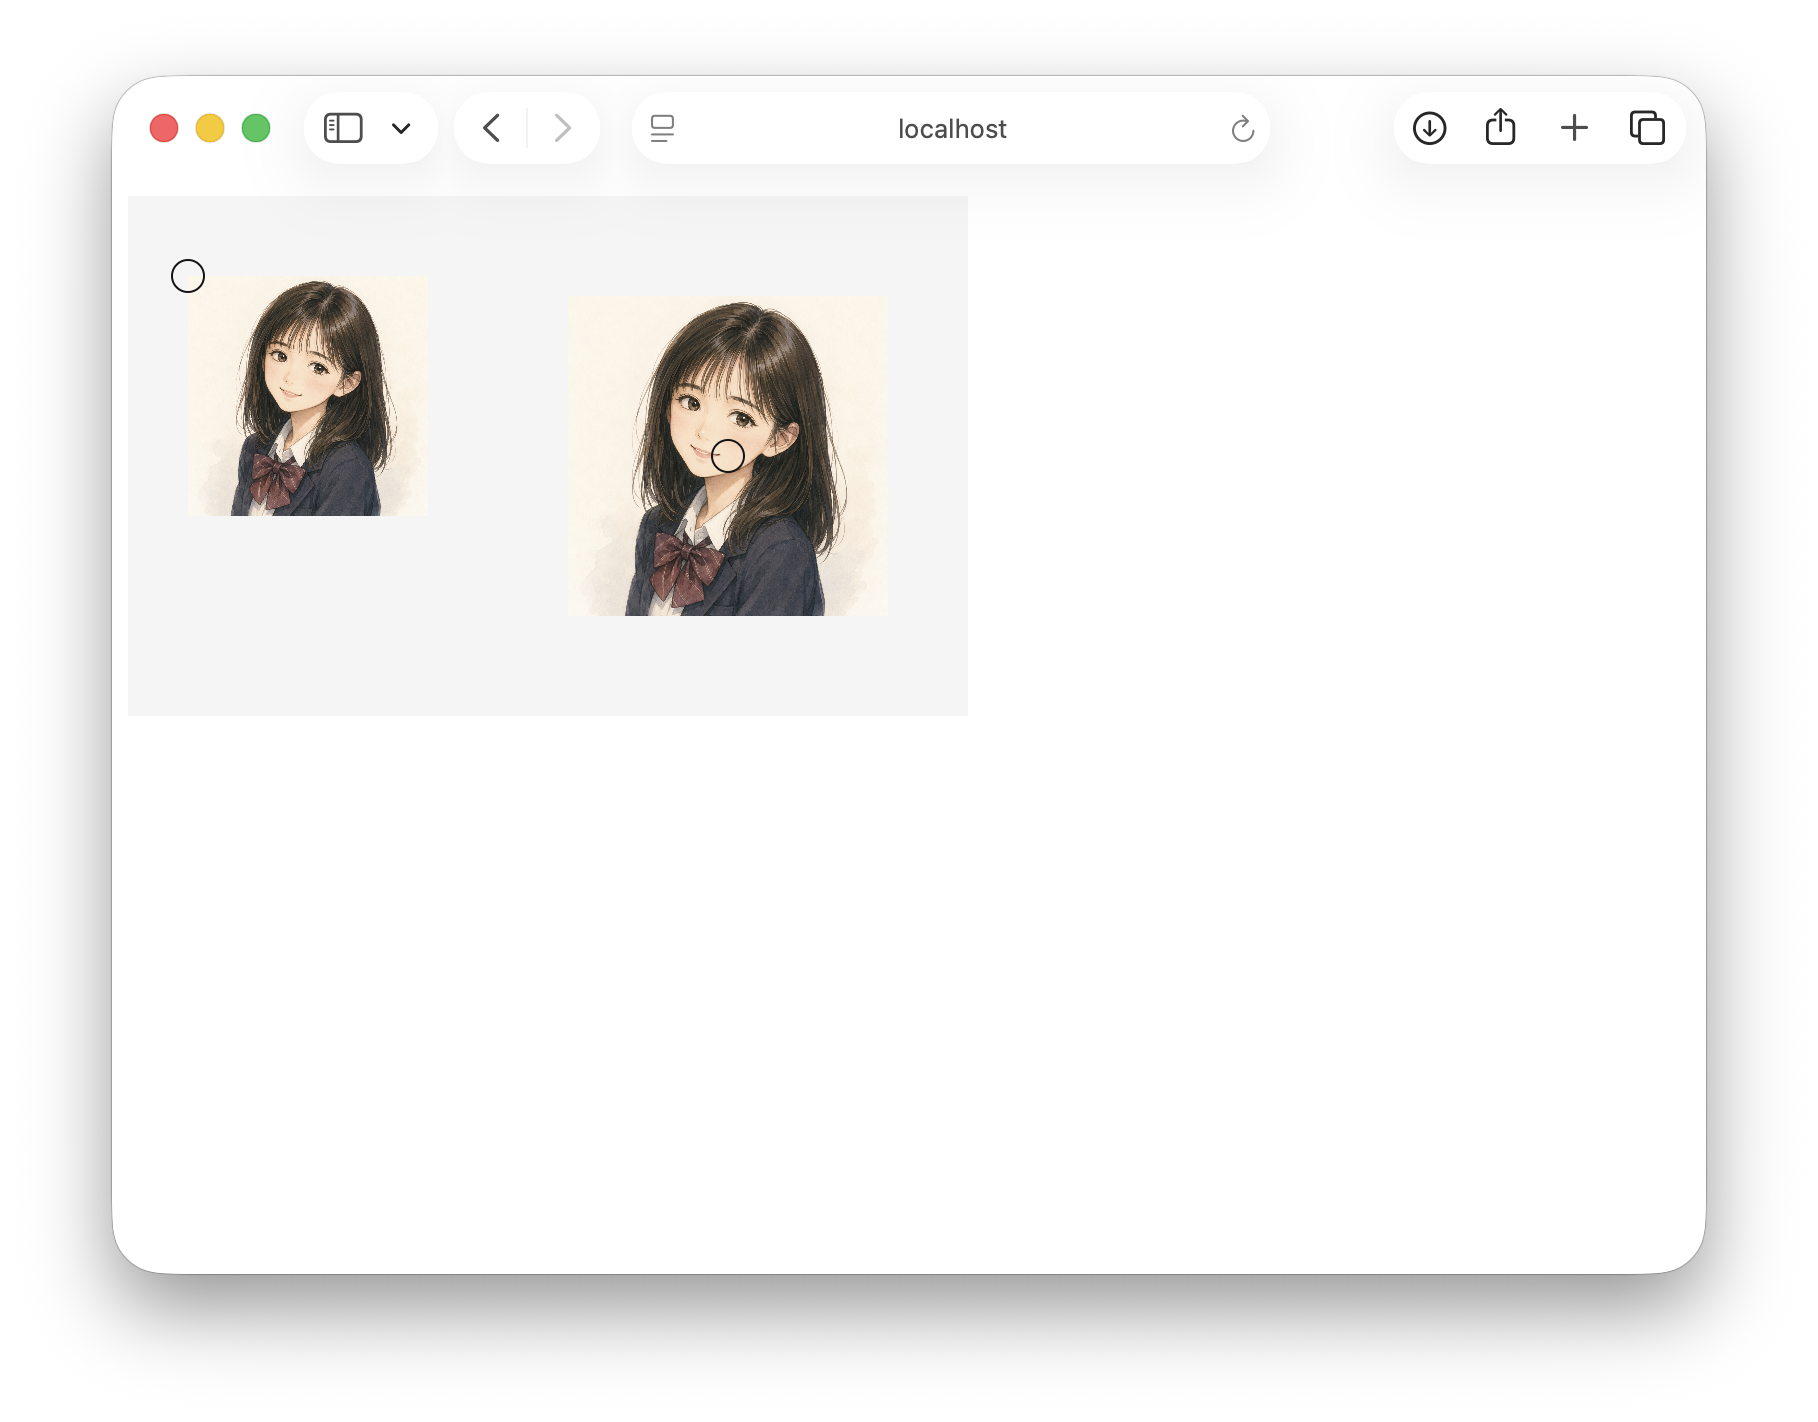
\includegraphics[
        width=0.70\linewidth,
        trim=50 331 419 35,
        clip
    ]{figures/chapter12/image-mode.png}
    \caption{\texttt{CORNER}と\texttt{CENTER}で座標の基準が変わる様子}
    \label{fig:chapter12-image-mode-result}
\end{figure}

図\ref{fig:chapter12-image-mode-result}の左側では、丸印の座標が画像の左上に一致しています。右側では、丸印の座標が画像の中心に一致しています。同じ座標を指定しても、\texttt{imageMode}によって画像が置かれる範囲が変わります。

\section{マウスで画像を動かす}

画像も、図形と同じように座標を変えることで動かせます。次のサンプルでは、画像をマウスの位置に表示し、マウスボタンを押している間だけ大きく表示します。

\begin{listing}[htbp]
\inputminted{ts}{listings/chapter12/image-follow-mouse.ts}
\caption{マウスの位置に画像を表示する}
\label{lst:chapter12-image-follow-mouse}
\end{listing}

\texttt{p.mouseIsPressed}は、マウスボタンが押されているかどうかを表す\texttt{boolean}型の値です。第6章で学んだ条件分岐を使えば、画像の大きさや表示位置を操作できます。

\begin{figure}[htbp]
    \centering
    \begin{minipage}[t]{0.47\linewidth}
        \centering
        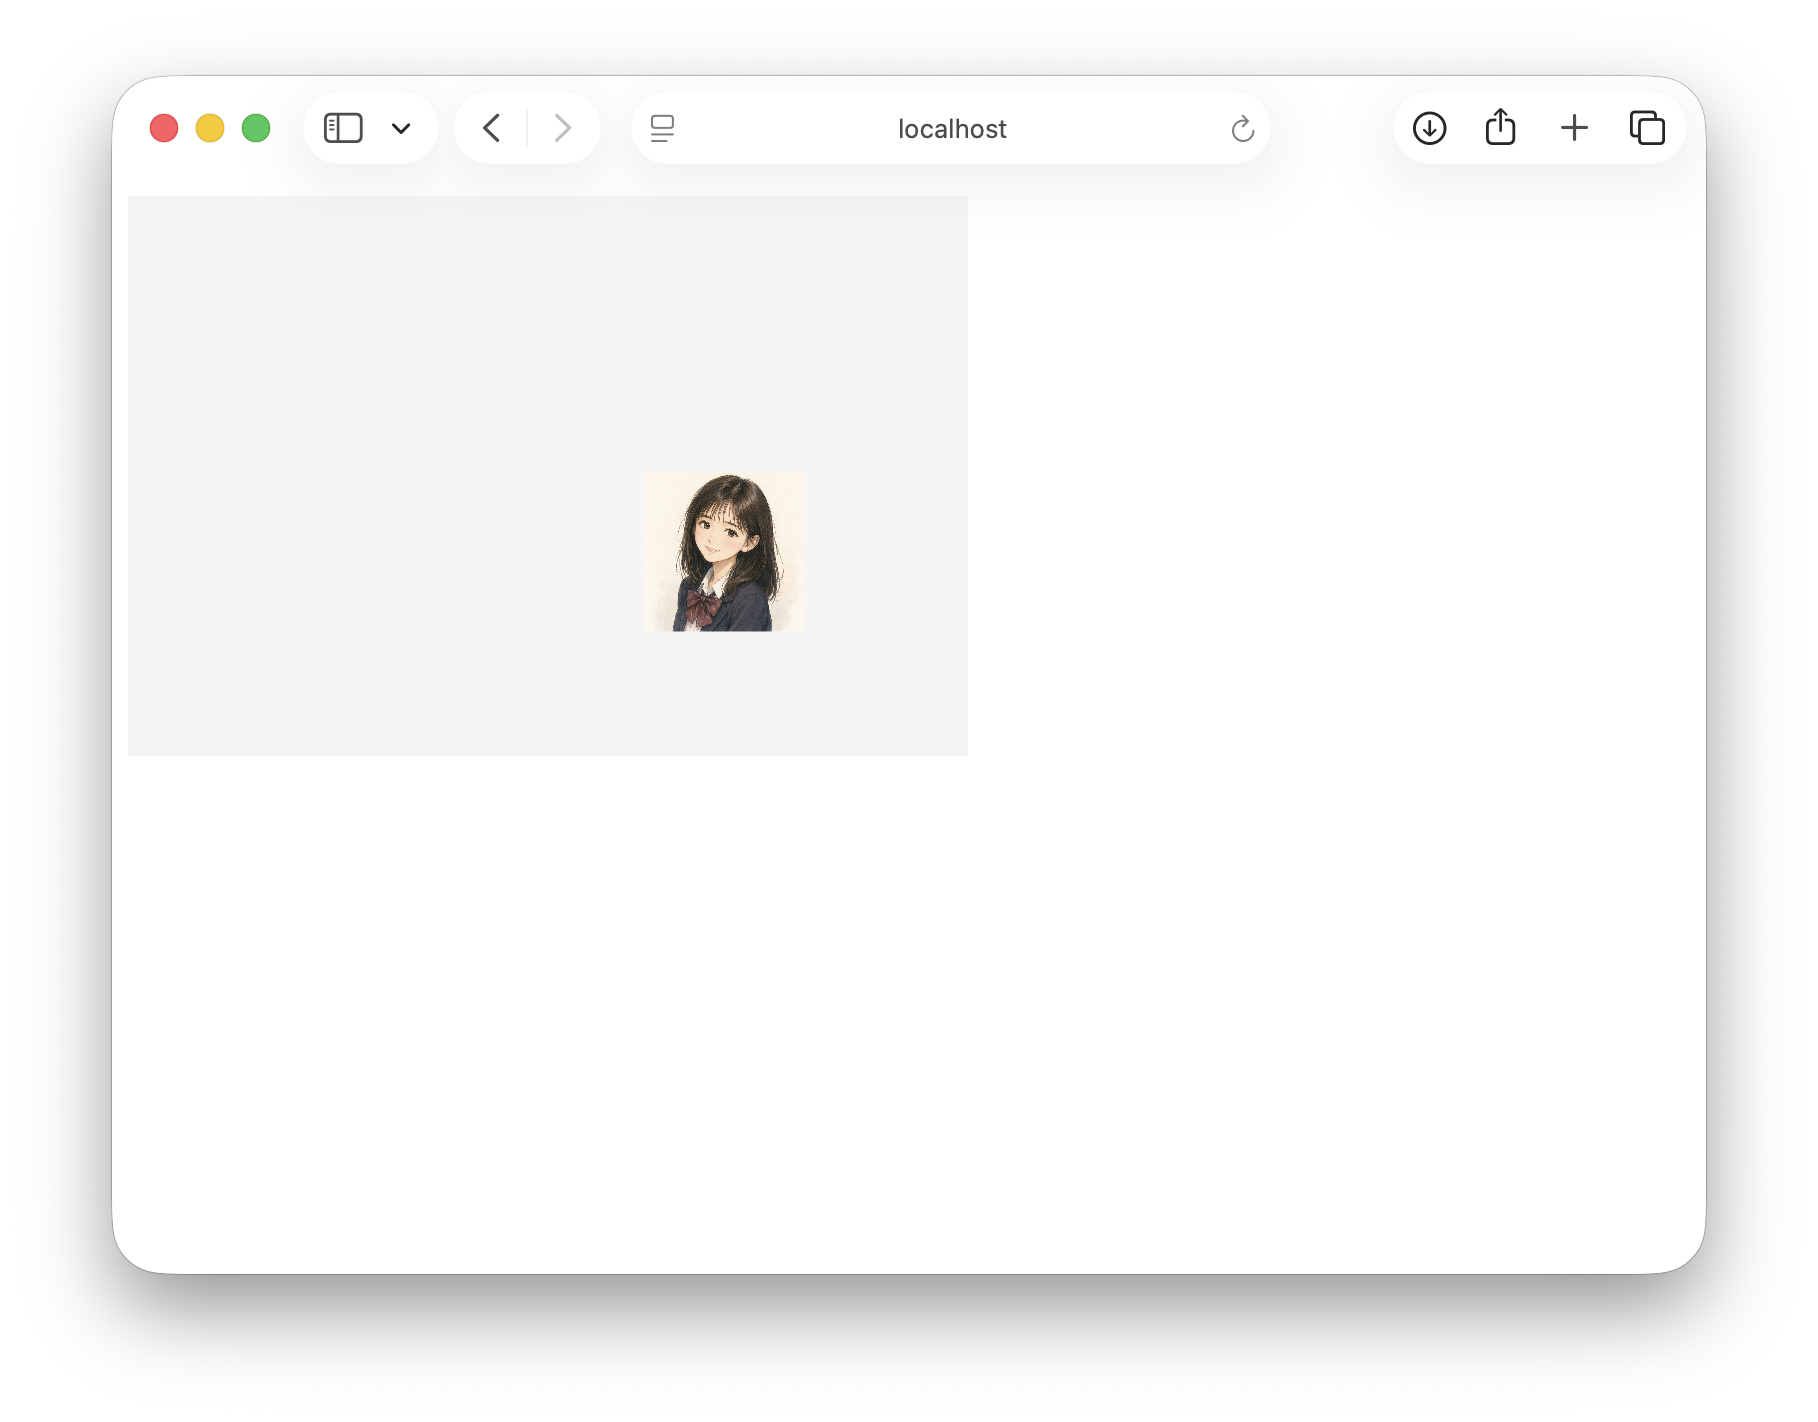
\includegraphics[
            width=\linewidth,
            trim=50 316 419 35,
            clip
        ]{figures/chapter12/follow-mouse-01.png}

        \small マウスを中央付近へ動かした場合
    \end{minipage}
    \hfill
    \begin{minipage}[t]{0.47\linewidth}
        \centering
        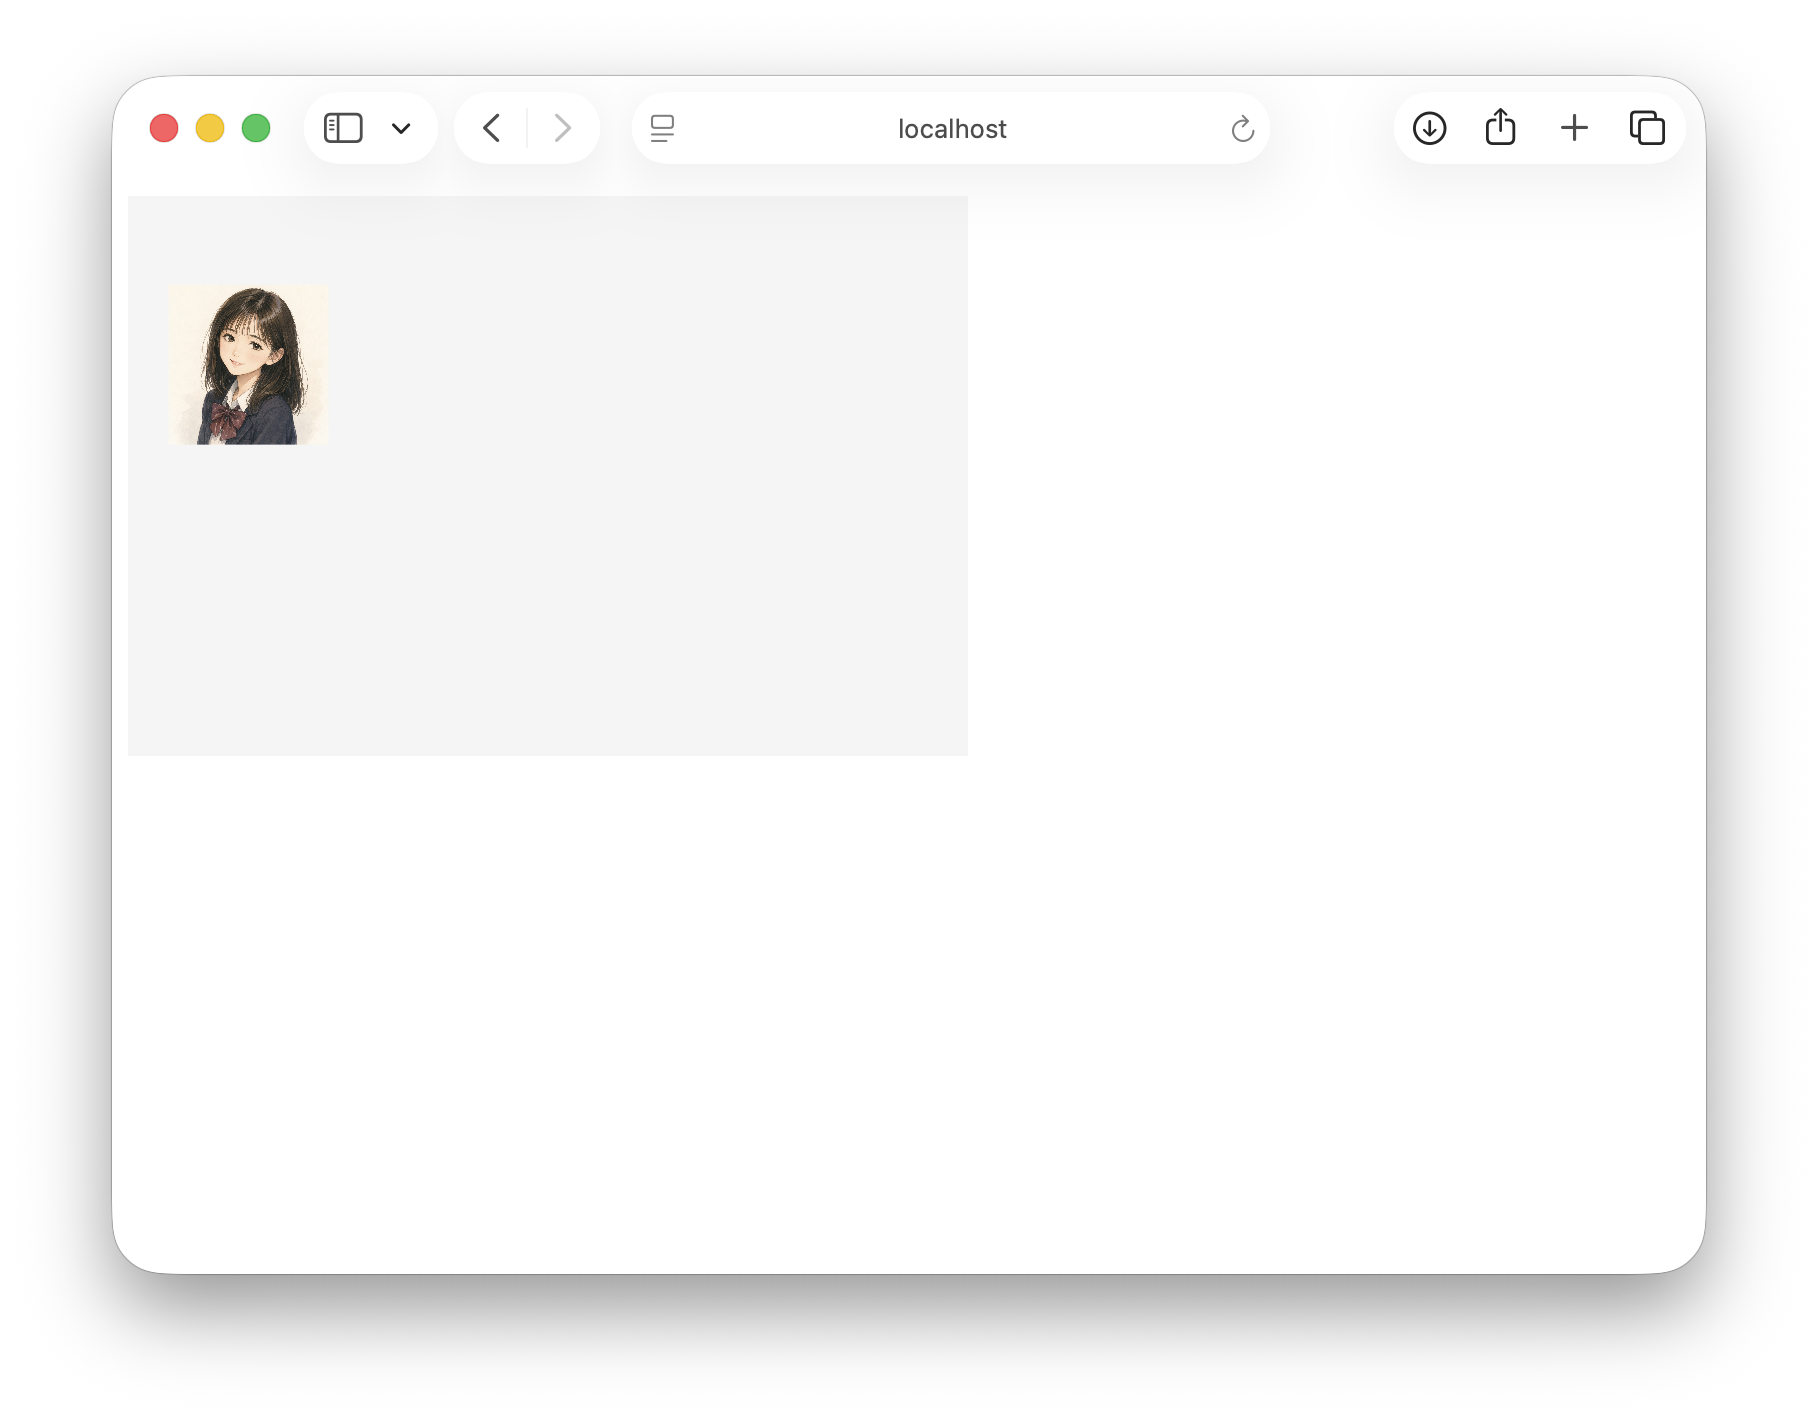
\includegraphics[
            width=\linewidth,
            trim=50 316 419 35,
            clip
        ]{figures/chapter12/follow-mouse-02.png}

        \small マウスを左上付近へ動かした場合
    \end{minipage}
    \caption{マウスの移動に画像が追随する様子}
    \label{fig:chapter12-follow-mouse-results}
\end{figure}

図\ref{fig:chapter12-follow-mouse-results}では、マウスを動かした前後の画面を並べています。\texttt{p.mouseX}と\texttt{p.mouseY}を画像の座標に使うことで、画像の中心がマウスの位置へ追随します。

\begin{pointbox}{画像も座標で動かせる}
画像は特別なものに見えますが、表示するときには座標と大きさを指定します。そのため、円や四角形と同じように、変数、条件分岐、繰り返し処理と組み合わせられます。
\end{pointbox}

\section{画像と文字を組み合わせる}

画像だけでなく、画像の上や下に文字を重ねると、カード、タイトル画面、ゲームの説明表示のようなものを作れます。描画順序はこれまでと同じで、後に描いたものほど手前に表示されます。

\begin{listing}[htbp]
\inputminted{ts}{listings/chapter12/image-caption-card.ts}
\caption{画像に説明文を重ねる}
\label{lst:chapter12-image-caption-card}
\end{listing}

このサンプルでは、最初に画像を描き、その後に半透明の長方形と文字を描いています。画像の上に読みやすい文字を置きたいときは、文字の背後に白や黒の半透明の長方形を置くと見やすくなります。

\begin{figure}[htbp]
    \centering
    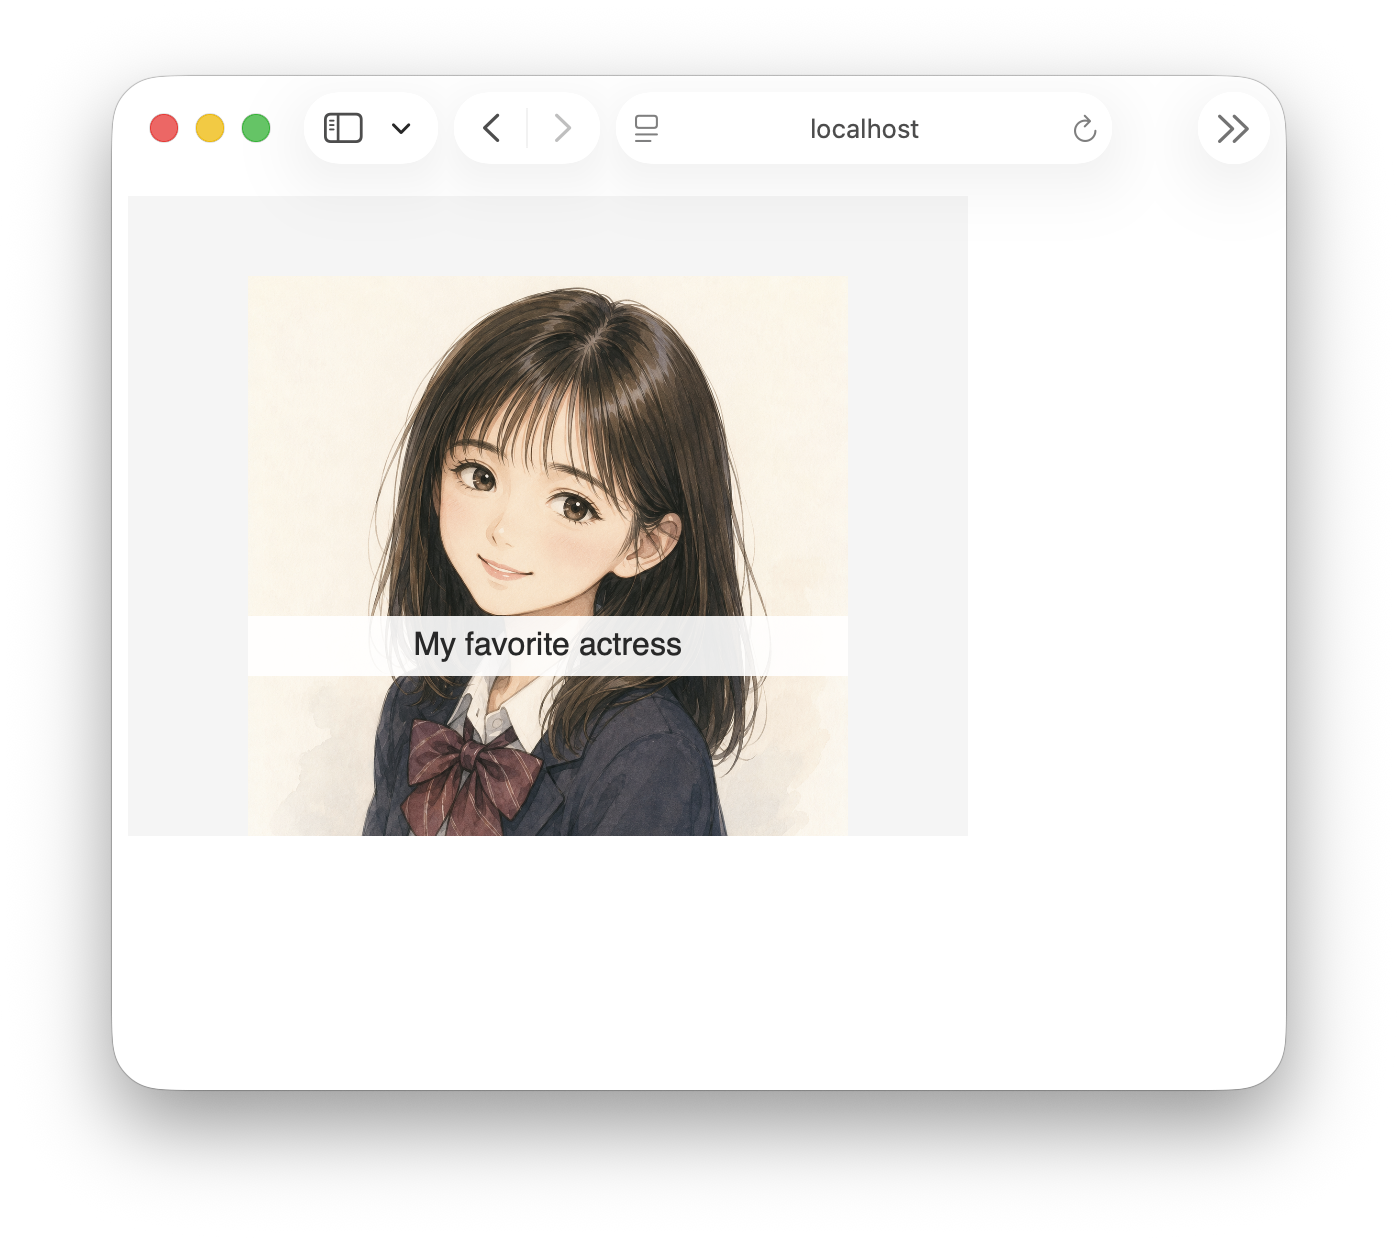
\includegraphics[
        width=0.62\linewidth,
        trim=50 179 204 35,
        clip
    ]{figures/chapter12/image-and-caption.png}
    \caption{画像の上へ半透明の長方形と文字を重ねた実行画面}
    \label{fig:chapter12-image-caption-result}
\end{figure}

図\ref{fig:chapter12-image-caption-result}では、画像を描いた後に半透明の白い長方形を描き、その上へ文字を描いています。文字の背後を少し明るくすることで、画像の色に左右されず説明文を読みやすくできます。

\begin{notebox}{描画順序を意識する}
文字を先に描いてから画像を描くと、画像が文字を隠してしまいます。背景、画像、文字のように、奥に置きたいものから順番に描きましょう。
\end{notebox}

\begin{notebox}{フォントを扱う順番}
まずはブラウザの標準フォントで文字を表示します。\texttt{p.textSize}は文字の大きさを、\texttt{p.textAlign}は文字の揃え方を設定します。特別な書体が必要になった段階で、Webフォントや\texttt{p.loadFont}を学びます。
\end{notebox}

\section{よくある間違い}

文字と画像では、ファイル名、描画順序、読み込みのタイミングでつまずきやすくなります。
エラーが出たときは、まず「ファイルの場所」「ファイル名」「\texttt{loadImage}で読み込んでいるか」
を確認しましょう。

\begin{mistakebox}{画像ファイルの場所や名前を間違える}
\texttt{p.loadImage("images/sample.png")}と書いた場合、実際にその場所に\texttt{sample.png}が必要です。大文字と小文字、拡張子、フォルダ名も一致させましょう。
\end{mistakebox}

\begin{mistakebox}{文字が画像に隠れる}
後から描いたものほど手前に表示されます。画像の上に文字を表示したい場合は、画像を描いた後に文字を描きます。
\end{mistakebox}

\begin{mistakebox}{\texttt{textAlign}の設定が残る}
\texttt{textAlign}の設定は、その後に描く文字にも影響します。別の場所で左揃えに戻したい場合は、\texttt{p.textAlign(p.LEFT, p.BASELINE)}のように設定し直します。
\end{mistakebox}

\section{まとめ}

この章では、文字列と画像を画面に表示する方法を学びました。文字列は\texttt{string}型で扱い、\texttt{text}、\texttt{textSize}、\texttt{textAlign}、\texttt{textWidth}を使って表示します。

画像は\texttt{p5.Image}型で扱い、\texttt{loadImage}関数を使って読み込みます。
ただし、\texttt{p.setup = async (): Promise<void> => \{ ... \};}のように、\texttt{async}を付けて書き、\texttt{loadImage}の前に\texttt{await}を付ける必要があります。

表示には\texttt{p.image}を使い、\texttt{imageMode}や表示サイズを指定することで、図形と同じように位置や大きさを制御できます。

\section{演習問題}

この章の演習では、文字と画像の表示を少しずつ変更しながら、作品の画面を作る練習をします。最初は文字列や座標を変えるだけでよいので、表示結果を確認しながら進めましょう。

\begin{enumerate}
    \item \texttt{basic-text.ts}の\texttt{message}を自分の好きな文字列に変更してください。
    \item \texttt{basic-text.ts}で、文字の色と大きさを変更してください。
    \item \texttt{text-align-box.ts}で、文字を左揃え、右揃えに変更して違いを確認してください。
    \item \texttt{moving-text.ts}で、文字列の移動速度を変えてください。
    \item \texttt{moving-text.ts}で、文字列が右から左ではなく、左から右へ動くようにしてください。
    \item \texttt{load-image-basic.ts}で、読み込む画像ファイル名を変更してください。
    \item \texttt{image-size-and-mode.ts}で、\texttt{p.CORNER}と\texttt{p.CENTER}の違いを説明してください。
    \item \texttt{image-follow-mouse.ts}で、マウスを押しているときに画像が小さく、離しているときに大きくなるようにしてください。
    \item \texttt{image-caption-card.ts}で、画像の下に表示する説明文を2行に増やしてください。
    \item 挑戦問題として、画像、タイトル、説明文、ボタン風の図形を組み合わせて、ゲームのタイトル画面を作ってください。
\end{enumerate}
